
\documentclass[a4paper,11pt,oneside]{Thesis}

\renewcommand{\contentsname}{Table of Contents}
\graphicspath{{Pictures/}{Figures/}}

\usepackage[square, numbers, comma, sort&compress]{natbib}
\usepackage{titlesec}
\titleformat{\chapter}[display]
  {\normalfont\bfseries}{}{0pt}{\Huge}
\usepackage{amsmath}

\usepackage{graphicx}
\usepackage[T1]{fontenc}

\usepackage{notoccite}

\usepackage{caption}
\usepackage{subcaption}
\usepackage{multirow}
\usepackage{longtable}
\usepackage{pdflscape}
\usepackage{array}
\newcolumntype{L}[1]{>{\raggedright\arraybackslash}p{#1}}
\usepackage{pifont}
\usepackage{hhline}
\usepackage{textcomp}

\usepackage{breqn}
\usepackage{rotating}
\usepackage{float}
\usepackage[ruled,vlined,linesnumbered]{algorithm2e}
\hypersetup{urlcolor=blue, colorlinks=true}
\title{\ttitle}

\begin{document}

\frontmatter

\setstretch{1.3}
\setlength{\emergencystretch}{3em}
\hbadness=10000

\fancyhead{}
\rhead{\thepage}
\lhead{}

\pagestyle{fancy}

\newcommand{\HRule}{\rule{\linewidth}{0.5mm}}

\hypersetup{pdftitle={\ttitle}}
\hypersetup{pdfsubject=\subjectname}
\hypersetup{pdfauthor=\authornames}
\hypersetup{pdfkeywords=\keywordnames}


\thispagestyle{empty}

\begin{center}
\begin{figure}
  \begin{center}
    
\includegraphics[height=4cm]{Pictures/logo}
  \end{center}
\end{figure}
\small
\textbf{ULM UNIVERSITY OF APPLIED SCIENCES\\
	FACULTY OF COMPUTER SCIENCE}

\vfill
\Large
\textbf{Thesis Title} \\

\vfill
\small
A thesis submitted in partial fulfillment of the requirements for the degree of\\
Master of Science in Computer Science \\

\vfill
\small
by\\
\large
\textbf{Mohamad Arabi}\\
\small

Computer Science\\
Faculty of Computer Science, Ulm University of Applied Sciences, 2026\\

\vfill
\small
\large
\textbf{April}\\
\textbf{2026}\\

\small

\vfill
\small
Supervised by\\
\normalsize
\textbf{Prof. Dr. Traub~\\
	  Prof. Dr. [Co-supervisor]~\\
	  }

\vfill
\small
Ulm, 2026\\

\end{center}




\cleardoublepage

\thispagestyle{empty}

\begin{center}\huge\textbf{Statement}\end{center}

\Large
\vfill
I hereby declare that this thesis is entirely the result of my own work except
where otherwise indicated. I have only used the resources given in the list
of references.

\vspace{1.5em}
\textbf{Use of AI} \\
AI tools were used to polish the text and improve the tone of this thesis. The ideas,
design, implementation, and evaluation are my own.

\vfill

\begin{flushright}
\large
\textbf{Mohamad Arabi} \\

\small
Signature \\
\dotfill\hspace{0.1 pt}

\textbf{Date:} 25 March, 2026 \\
\end{flushright}
\vfill

\normalsize



\cleardoublepage
\newpage
\thispagestyle{empty}

\phantomsection
\addtotoc{Abstract}

\begin{center}\huge \textbf{Abstract}\end{center}
\noindent Security operations teams are flooded with alerts, and most SIEM platforms still leave triage and response to human analysts. This thesis presents a generic SIEM reaction plugin that adds a reasoning layer on top of normal SIEM output, with explicit focus on security rule enforcement and compliance-oriented checks in cloud-connected environments. Alerts are normalized, enriched, scored with an explainable risk model, and passed to a planner that produces structured response plans. Each plan is checked by policy rules before any action is executed, and every step is recorded in an audit log.
\par\noindent The system is implemented as a single runnable project with a reasoning-focused interface that shows the full chain: raw alert, normalized alert, score and evidence, plan, policy decision, and execution result. The evaluation uses synthetic and public security datasets and shows strong planning accuracy with consistent, explainable outputs. The result is a practical foundation for moving from rule-heavy SIEM workflows to reasoning-driven response that is auditable, safe, and easy to extend.



\cleardoublepage
\newpage
\thispagestyle{empty}
\phantomsection
\addtotoc{Summary}

\begin{center}\huge \textbf{Summary}\end{center}

\vfill

\begin{flushleft}
\large

Security operations centres face a structural gap between detection and response. SIEM
platforms collect, correlate, and surface alerts---but what happens next remains a manual
decision. Commercial SOAR tools execute pre-scripted playbooks, which break down on
novel attack patterns and cannot reason about threat severity or asset criticality.

This thesis fills that gap with an intelligent reaction layer that sits downstream of a
SIEM and upstream of any action. The system takes a normalised alert, enriches it with
asset, identity, and threat-intelligence context, produces an explainable threat
assessment, generates a structured response plan, and passes every proposed action
through a deterministic policy engine before execution. All decisions are recorded in a
structured audit log linking each action to its evidence.

The architecture is a modular monolith: a C\# core engine enforces the orchestration
pipeline and safety constraints, while a Python intelligence service provides scoring
and planning via HTTP. The threat scorer combines TF-IDF logistic regression with
contextual enrichment boosts. The planner is a custom 270K-parameter multi-head neural
network that classifies strategy, predicts action sets, and regresses priority---
resolving entity parameters deterministically rather than generating them, eliminating
the hallucination risk that made LLM-based planning unsafe for live execution.

The planner achieves 96.4\% strategy accuracy and 97.2\% action F1 in end-to-end
pipeline evaluation---matching a 250-million-parameter fine-tuned seq2seq model at
under 5 milliseconds inference time. The policy engine guarantees that no model error
can cause a hard-denied action to execute. The full system runs on a single development
machine and exposes every stage of the decision pipeline for analyst review.

\end{flushleft}



\cleardoublepage
\newpage
\thispagestyle{empty}
\phantomsection
\addtotoc{Acknowledgment}

\begin{center}\huge \textbf{Acknowledgment}\end{center}

I would like to express my deepest appreciation to all those who contributed to the
successful completion of my master's thesis. Foremost, I extend my heartfelt
appreciation to my esteemed advisor, Prof. Dr.-Ing. Traub. His guidance, insights,
counsel, and mentorship were instrumental in shaping this research.

I also thank Prof. [Second Examiner], who graciously served as the second examiner.
Lastly, I would like to thank all individuals and resources, too numerous to name,
who contributed indirectly through their research, books, articles, and online sources.

\vfill
\begin{flushright}
\large
Mohamad Arabi\\
Department of Computer Science\\
Technische Hochschule Ulm\\
Ulm, Germany\\
15 April, 2026
\end{flushright}


\clearpage
\pagestyle{fancy}

\lhead{\emph{Table of Contents}}
\tableofcontents

\clearpage
\lhead{\emph{List of Figures}}
\listoffigures

\clearpage
\phantomsection
\lhead{\emph{List of Tables}}

\addtotoc{List of Tables}
\listoftables

\clearpage

\lhead{\emph{List of Abbreviations}}

\clearpage
\listofsymbols{ll}
{

\textbf{SIEM} & \textbf{S}ecurity \textbf{I}nformation and \textbf{E}vent \textbf{M}anagement \\
\textbf{SOAR} & \textbf{S}ecurity \textbf{O}rchestration, \textbf{A}utomation, and \textbf{R}esponse \\
\textbf{SOC} & \textbf{S}ecurity \textbf{O}perations \textbf{C}enter \\
\textbf{EDR} & \textbf{E}ndpoint \textbf{D}etection and \textbf{R}esponse \\
\textbf{XDR} & e\textbf{X}tended \textbf{D}etection and \textbf{R}esponse \\
\textbf{IOC} & \textbf{I}ndicator \textbf{o}f \textbf{C}ompromise \\
\textbf{TTP} & \textbf{T}actics, \textbf{T}echniques, and \textbf{P}rocedures \\
\textbf{ATT\&CK} & Adversarial \textbf{T}actics, \textbf{T}echniques, and \textbf{C}ommon \textbf{K}nowledge \\
\textbf{LLM} & \textbf{L}arge \textbf{L}anguage \textbf{M}odel \\
\textbf{ML} & \textbf{M}achine \textbf{L}earning \\
\textbf{JSON} & \textbf{J}ava\textbf{S}cript \textbf{O}bject \textbf{N}otation \\
\textbf{API} & \textbf{A}pplication \textbf{P}rogramming \textbf{I}nterface \\
\textbf{STIX} & \textbf{S}tructured \textbf{T}hreat \textbf{I}nformation e\textbf{X}pression \\
\textbf{TAXII} & \textbf{T}rusted \textbf{A}utomated e\textbf{X}change of \textbf{I}ndicator \textbf{I}nformation

}

\clearpage

\lhead{\emph{List of Symbols}}

\listofnomenclature{lll}
{
$R$ & risk score (overall) \\
$b$ & bias term in risk model \\
$w_i$ & feature weight $i$ \\
$x_i$ & feature value $i$ \\
$m$ & context multiplier \\
$c$ & confidence (0--1) \\
$S$ & severity (0--100) \\
$P$ & response priority (0--100)

}

\mainmatter

\pagestyle{fancy}

\chapter{Introduction}
\label{chap:introduction}

\lhead{\emph{Introduction}}

\section{Motivation}

Security Operations Centers (SOCs) rely on SIEM platforms to collect and centralize security logs from many different systems. \cite{nist80092} Theoretically, this should allow analysts to have a complete view of what is going on with the infrastructure. In practice, the SOC analysts deal with a constant flow of alerts. Many of them are noisy, duplicated, and of poor quality. Moreover, they still need to be examined and the decision made which ones actually signal a threat.\cite{ban2023alertfatigue}

This situation creates several problems. Alert queues accumulate quickly, response time increases, and the analyst works under the pressure of the possibility that an important alert will be missed.  This leads to a phenomenon referred to as alert fatigue, where the information overload is more challenging to deal with than the actual issues themselves.\cite{tilbury2024humans}

To understand this, let's consider an example. For instance, if there are several unsuccessful login attempts, it may be indicative of a brute-force attack. However, it may also be indicative of a misconfigured script. A human analyst will be able to understand the difference between the two, but only if the necessary context is provided and it is presented in an understandable manner. So, it's not just the matter of detecting, but it's also about reasoning, prioritization, and determining the course of action.
\section{Problem Statement}

Most SIEM environments rely on rule-based detection. As rule sets gets bigger over time, they tend to overlap and produce redundant alerts. This increases the workload and makes it harder to identify the alerts that actually require attention. \cite{rulegenie2025} Even in environments that introduce automation, studies show that SOC workflows still depend a lot on human judgment when deciding how to respond to incidents. \cite{tilbury2024humans}

This creates a gap in current SIEM workflows. While SIEM platforms are effective at collecting and detecting events, they provide limited support for reasoning about response actions.While alerts are generated, the system generally does not create a plan for what should be done next. Additionally, there is no capturing of analyst feedback to improve future decisions.

This thesis attempts to fill this gap by proposing a generic reaction layer. This layer will be used after the alert normalization process. It will evaluate the alerts, create explainable risk scores, and create a plan for the response. The policy will be used before the actions are taken, and an audit trail will be used for the decisions.
\section{Research Objectives}

The work presented in this thesis is guided by the following objectives:

\begin{itemize}
    \item Design a layered architecture that separates orchestration from intelligence and allows detection models to be replaced without disrupting the surrounding SIEM pipeline.
    
    \item Implement an explainable risk scoring engine that uses evidence-based features
along with contextual information and offers an explanation for each score.
    \item  Create a structured planning module that offers response plans, policy
conformance for those plans, and rollbacks.
    \item Integrate analyst feedback and investigation traces so that the system can learn from past investigations and suggest useful next steps.
    
    \item Demonstrate the approach through an end-to-end prototype that includes a runnable system and an interface focused on reasoning and investigation support.
\end{itemize}

\section{Thesis Structure}

The remainder of this thesis is organized as follows. Chapter 2 reviews background concepts and related work in SIEM systems, alert correlation, and response automation. Chapter 3 defines the system requirements. Chapter 4 explains the system design and architecture. Chapter 5 explains the implementation
details of the system. Chapter 6 explains the dataset pipeline and the training
approach used for the models. Chapter 7 explains the evaluation of the system. It
includes the results of the system. Chapter 8 explains the implications of the system.
Finally, Chapter 9 concludes the thesis. It explains the possible directions for
future work.
\chapter{Background and Related Work}

\label{chap:background-related-work}

\lhead{\emph{Background and Related Work}}

% -----------------------------------------------------------------------------
\section{Cybersecurity Monitoring and Security Operations Centers}

Modern organisations generate massive volumes of digital events. These include network flows, logins, process executions, and file system changes. A Security Operations Center (SOC) is responsible for monitoring this activity, triaging suspicious events, and coordinating response.

The classic incident response lifecycle is documented by NIST in SP 800-61. \cite{nist80061} It separates work into preparation, detection and analysis, containment and recovery, and post-incident review. The detection and analysis phase is usually the most expensive because it depends on human interpretation and on the quality of monitoring infrastructure.

SOC teams operate under high pressure. Tilbury and Flowerday report sustained alert overload and a tension between automation and human oversight. \cite{tilbury2024humans} Their conclusion is practical: automation should reduce mechanical workload, not remove human judgment from high-impact decisions. This thesis follows that principle.

% -----------------------------------------------------------------------------
\section{Security Information and Event Management (SIEM)}

\subsection{Log Collection and Normalization}

A SIEM platform collects logs from heterogeneous sources and makes them queryable for analysts and correlation engines. NIST SP 800-92 describes SIEM log management as a pipeline: collect, parse, normalize, and store. \cite{nist80092}

Normalization is a core requirement. Windows Event Logs, syslog, CEF, and LEEF all use different field layouts. A field called \texttt{severity} in one source can mean an alert priority, while in another it reflects a risk assessment. Normalization mistakes propagate into every downstream stage. For that reason, the system in this thesis treats normalization as a separate, explicit pipeline stage that can be updated without touching the intelligence layer. This aligns with the modularity principle in \cite{nist80092}.

\subsection{Event Correlation}

Single events are rarely enough. A single failed login is usually noise, but many failed logins in a short time can indicate brute force. Correlation connects events across time and sources to create a higher-level alert.

Valeur et al. \cite{valeur2004alert} describe correlation as a structured process: preprocessing, duplicate removal, alert fusion, correlation, false-positive reduction, and session reconstruction. Their work highlights a practical issue: what practitioners call ``correlation'' is often several different operations mixed together. Separating these stages makes the system easier to reason about and improves control over false positives.

\subsection{Alerting and Incident Response}

The output of correlation is an alert. An analyst must decide whether it is real, how severe it is, and what response is appropriate. The process is formalized in \cite{nist80061}, but in practice prioritization varies by analyst and by workload. \cite{tilbury2024humans} This inconsistency motivates machine-assisted scoring and structured response planning.

% -----------------------------------------------------------------------------
\section{Limitations of Current SIEM Systems}

\subsection{Rule-Based Detection}

Rule-based correlation does not generalize. Rules encode what an expert anticipated, but they fail on novel or subtle patterns. Attackers exploit this with ``living-off-the-land'' techniques that use legitimate tools (PowerShell, WMI, certutil) to avoid signatures. \cite{strom2018attack}

Rule sets also accumulate and overlap. Sarhan et al. show that redundant rules generate unnecessary alerts and that rule hygiene has a measurable effect on alert quality. \cite{rulegenie2025} This is not only a volume problem; it is a correctness problem.

\subsection{Alert Overload and False Positives}

High false-positive rates lead directly to alert fatigue. Ban et al. report deployments where false positives dominate the alert stream, forcing analysts to ignore alerts just to keep up. \cite{ban2023alertfatigue}

Axelsson's base-rate analysis explains why this is structural. \cite{axelsson2000baseratev} Even a detector with 99\% sensitivity and 99\% specificity can produce more false alerts than true alerts when the base rate of attacks is low. This makes precision a central requirement for any operational system.

\subsection{Scalability and Data Volume}

Enterprise log volume can reach terabytes per day. \cite{nist80092} Scaling ingestion is possible, but it does not reduce analyst workload. Alert volume depends on rule behavior and correlation quality. \cite{rulegenie2025} Without better reasoning, more data simply means more alerts.

\subsection{Dependence on Human Analysts}

SOC effectiveness is still bounded by human availability. Tilbury and Flowerday describe analyst shortage, turnover, and burnout as persistent constraints. \cite{tilbury2024humans} This reinforces the need for systems that handle mechanical triage while preserving human control of high-impact decisions.

% -----------------------------------------------------------------------------
\section{Machine Learning Approaches to Intrusion Detection}

Rule limitations have driven research into machine learning for intrusion detection and alert analysis. Two main paradigms dominate the literature.

\textbf{Anomaly-based detection} learns a model of normal behavior and flags deviations. Garcia-Teodoro et al. survey anomaly detection methods and show that while these systems can detect novel attacks, they often generate high false-positive rates because ``abnormal'' includes many benign but unusual behaviors. \cite{garcia2009anomaly}

\textbf{Signature-based ML} treats detection as a classification problem trained on labeled attacks. This can produce high precision for known patterns but struggles on new attack variants, similar to rules.

Sommer and Paxson provide a critical analysis of ML for network intrusion detection. \cite{sommer2010outside} They argue that distribution shift, attacker adaptation, and data quality issues limit the operational reliability of ML systems. Their critique motivates the design of systems that emphasize explainability, policy constraints, and bounded automation rather than blind reliance on model accuracy.

% !TeX root = ../main.tex
\chapter{System Requirements}
\label{chap:system-requirements}
\lhead{\emph{System Requirements}}

\section{Functional Requirements}

The system ingests alerts from external SIEM sources, normalises them to a common schema, enriches them with contextual data, and produces ranked incident candidates. For each incident the scoring component generates an explainable risk score and confidence value, accompanied by reason codes and context multipliers. The planning component then produces a structured response plan---strategy, priority, action set, and rollback steps---which is validated against explicit policy rules and compliance-oriented checks before any action is dispatched. The execution stage records action outcomes and errors.

Analyst feedback is a first-class input. An analyst can mark an incident as true positive, false positive, or needs more information, and optionally override severity. Feedback events are recorded in an append-only log and used to update model weights in a bounded, auditable way. Investigation traces are tracked and used to recommend next steps. A user interface exposes raw alerts, normalised alerts, scoring explanations, plans, policy checks, execution status, and audit logs.

Figure~\ref{fig:req-traceability} provides a requirement-to-component traceability view,
showing where each requirement class is enforced in the architecture.

\begin{figure}[H]
  \centering
  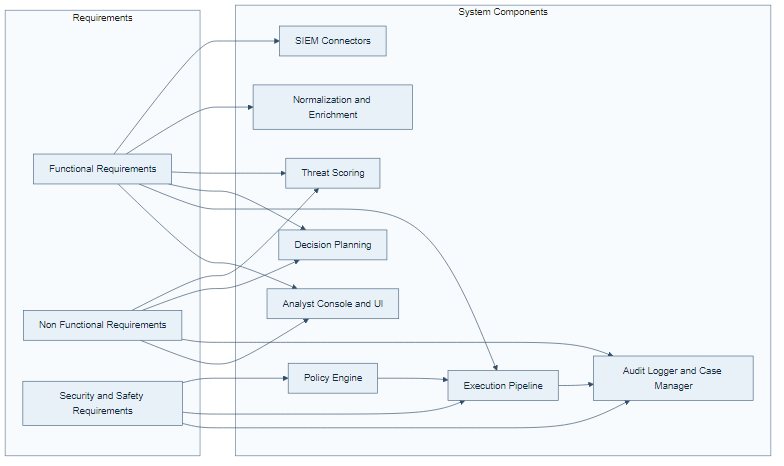
\includegraphics[width=\textwidth]{Diagrams/Requirements_Traceability.png}
  \caption{Traceability mapping from functional, non-functional, and safety requirements to core system components.}
  \label{fig:req-traceability}
\end{figure}

\section{Non-Functional Requirements}

The architecture is modular so that intelligence models can be swapped without touching orchestration code. The interface between layers is explicit and versioned. The system must run as a single project to facilitate demonstrations and repeated experiments. Explanations are human-readable and consistent across alerts to allow direct comparison.

There is a clear separation between domain logic, application services, infrastructure, and the UI. Structured logging throughout facilitates audits and retrospective analysis.

\section{Security and Safety Requirements}

Automation is bounded by design. All planner actions are subject to policy rules---allow/deny lists, confidence thresholds, asset criticality limits. High-impact actions require approval gates, and each automated action has a corresponding rollback. The execution layer validates parameters, enforces entity-presence checks, and refuses to execute when required context is missing or policy checks fail. Rate limits and idempotency safeguards prevent repeated execution under noisy alert conditions.

If confidence is too low or policy approval is not granted, the system falls back to recommendation-only behaviour. Model risk is controlled through bounded, logged weight updates. Model output is traceable after updates, and the system supports drift detection and periodic offline recalibration. Connectors and executors operate under least-privilege access, and sensitive fields are minimised or redacted where possible. All policy evaluations and execution outcomes are logged with timestamps and actor identity.

\chapter{System Design and Architecture}
\label{chap:system-architecture}
\lhead{\emph{System Design and Architecture}}

% -----------------------------------------------------------------------------
\section{Design Goals}

The architecture was built around a small set of goals that reflect how SOC systems are used in practice.

\textbf{Explainability first.} Every score, strategy, and action must have a reason that an analyst can read. This rules out black-box outputs and forces the system to carry evidence and rationale at every stage.

\textbf{Safety before speed.} A wrong containment action can be worse than a missed alert. The design therefore enforces policy checks and approval gates before execution, even if that adds latency.

\textbf{Modularity and replaceability.} Models and connectors change quickly. Each component must be swappable without rewriting the rest of the pipeline.

\textbf{Runs on one machine.} The system must be runnable end-to-end on a single developer machine for demos and testing. External services are optional, not required.

\textbf{Reproducibility.} Given the same input and configuration, the system should produce the same output. This requires deterministic post-processing and a clear audit trail.

% -----------------------------------------------------------------------------
\section{Key Architectural Decisions}

\subsection{Modular Monolith over Multi-Agent Architecture}

A multi-agent design was considered. It would split ingestion, scoring, planning, and execution into separate autonomous agents. While this can scale, it introduces distributed failure modes and makes reasoning harder to audit. In security response, accountability matters more than autonomy. For that reason, the core engine is a modular monolith with a single, synchronous pipeline. Every decision flows through one call chain that can be logged end-to-end.

\subsection{Two-Process Boundary: C\# Orchestration and Python Intelligence}

The system is intentionally split into two processes. The orchestrator runs in C\# (.NET) because it handles state, policy enforcement, and long-running reliability. The intelligence service runs in Python because the ML ecosystem lives there. The two communicate over HTTP with a strict JSON contract. This boundary keeps each side simple: the orchestrator stays stable, and the intelligence layer can evolve quickly.

\subsection{Interface-Driven Design}

Each stage is defined by an interface: connector, normalization pipeline, scorer, planner, policy engine, execution pipeline, audit logger, and case manager. This makes the
system testable with stubs and components replaceable without modifying the orchestrator.

\subsection{Policy as a Local, Synchronous Gate}

Policy evaluation is inside the core engine, not a remote call. This guarantees that no action can bypass safety checks due to network failures or model errors. Hard denials are applied before any approval workflow, which prevents unsafe actions from entering the approval queue.

\subsection{Structured Prediction over Free-Form Planning}

Early experiments with free-form JSON planning showed two problems: invalid output and hallucinated entities. The system therefore treats planning as structured prediction. The model selects a strategy and action types, while entity parameters are filled deterministically from the normalized alert. This removes hallucination by design.

% -----------------------------------------------------------------------------
\section{System Overview}

The system processes alerts in a linear pipeline:

\begin{verbatim}
Ingest -> Normalize -> Enrich -> Score -> Plan -> Policy -> Execute -> Audit
\end{verbatim}

Each stage emits structured data and is logged. The pipeline is synchronous and deterministic, which makes it easier to explain and to debug.

% -----------------------------------------------------------------------------
\section{Event Ingestion Layer}

The ingestion layer pulls alerts from external SIEMs or accepts them via webhook. Two connectors are implemented: a Wazuh connector for real SIEM input and a simulator for controlled demos. Each connector outputs a \texttt{RawAlert} object with the original payload and metadata such as source, alert ID, and timestamp.

% -----------------------------------------------------------------------------
\section{Normalization and Enrichment}

Normalization transforms non-uniform alert data formats to a standardized format.
Consider the Wazuh alert format that stores the IP address of the source in data.srcip,
and the Sentinel alert format that stores the IP address of the source as a list of
entities. The mapping registry normalizes these differences.
Enrichment provides contextual information like criticality of assets, threat intel hits,
and identity privileges. These fields are optional; if an enrichment source is missing, the system continues with null values rather than failing the entire pipeline.

% -----------------------------------------------------------------------------
\section{Threat Scoring Component}

The scoring stage produces a \texttt{ThreatAssessment} with severity, confidence, hypothesis, and evidence. The default scorer is a TF-IDF based classifier with calibrated confidence thresholds. A hybrid mode can add an LLM explanation when confidence is borderline. A rule-based fallback ensures that the pipeline always returns a score.

The scorer is informational, not authoritative. Its output drives planning and policy, but policy rules can still block actions even for high scores.

% -----------------------------------------------------------------------------
\section{Decision Planning Component}

Planning converts an assessment into a structured \texttt{DecisionPlan}. Each plan includes a strategy, priority, a list of actions, and rationale text. The system uses five strategy labels:

\begin{itemize}
  \item \textbf{Ignore}: The alert is assessed as benign noise; no action is taken.
  \item \textbf{NotifyOnly}: Low severity or confidence; notify the SOC and open a ticket.
  \item \textbf{Investigate}: Warrants investigation but no automated containment.
  \item \textbf{ContainAndCollect}: Active threat confirmed; containment plus forensics.
  \item \textbf{Contain}: Immediate high-confidence threat; containment is the priority.
\end{itemize}

The planner is model-driven, but its output is sanitized to enforce schema validity, safe actions at low confidence, and parameter completeness. This keeps the plan consistent even when models fail or return partial output.

% -----------------------------------------------------------------------------
\section{Policy and Safety Layer}

The policy engine analyzes each proposed action and returns a decision of Approved, Pending,
or Denied. Hard constraints are checked first (missing entities, forbidden actions, low confidence).
Approval gates are applied next, using risk, environment, and asset criticality factors. All policy
decisions are logged with explanations so that analysts can trace exactly why a particular action
was allowed or denied.
% -----------------------------------------------------------------------------
\section{Action Execution and Response}

Approved actions are routed to executors (ticketing, notification, firewall, host isolation). Each executor validates parameters and returns a structured result. In demo mode, executors simulate the action and only write audit entries. This keeps the system safe while still showing a complete execution pipeline.

% -----------------------------------------------------------------------------
\section{Audit and Explainability Components}

Every stage writes structured audit events to JSONL. These logs include the raw alert, normalized alert, assessment, plan, policy decision, and execution results. The same data powers the reasoning console UI, which allows the full decision trail to be viewed and replayed.

% -----------------------------------------------------------------------------
\section{Cross-Cutting Concerns}

\textbf{Configuration.} All services are configured via environment variables and a single \texttt{.env} file, making model switching and demo setup fast.

\textbf{Resilience.} Each stage is isolated; a failure in one alert does not crash the pipeline for the entire batch.

\textbf{Extensibility.} New connectors, actions, or models can be added by implementing a single interface and registering it with the container or model registry.

\chapter{Implementation}
\label{chap:implementation}
\lhead{\emph{Implementation}}

Building a system that reasons about security threats is, at its core, an exercise in managing complexity across layers that evolve at very different speeds. The orchestration layer must be rock-solid and deterministic --- it cannot afford to crash when a model fails or a network call times out. The intelligence layer, on the other hand, needs to be fluid: models get retrained, thresholds get tuned, and entirely new backends can be swapped in overnight. Getting this boundary right was one of the first and most consequential decisions in the implementation.

This chapter walks through every major component of the system, explaining not just what was built but why each decision was made the way it was. The intent is to give a software engineer enough context to understand, reproduce, or extend any part of the implementation without needing to reverse-engineer intent from code alone.

% -----------------------------------------------------------------------------
\section{Technology Stack}
\label{sec:impl-stack}

The system is split into two cooperating services with distinct runtime requirements, and the technology choices reflect that distinction honestly.

\subsection{Orchestration Layer: .NET 9 / C\#}

The orchestration engine is written in C\# and targets \texttt{net9.0}. C\# was chosen because it provides strong static typing, high-performance async I/O, and a mature dependency injection container. These are not incidental features --- they are the specific properties the orchestration layer needs. Strong typing catches interface contract violations at compile time. Async I/O allows concurrent enrichment lookups without thread-per-request overhead. The DI container wires the pipeline together with minimal ceremony and makes it trivial to swap any component.

The decision not to use a full web application framework like ASP.NET was deliberate. The engine runs as a console application, not a web server, because its job is to process alerts, not to serve HTTP requests. The webhook \emph{listener} is a small HTTP utility used only in webhook mode --- the engine remains a pipeline, not a service.

\subsection{Intelligence Layer: Python / FastAPI}

The intelligence service is implemented as a Python \texttt{FastAPI} application. Python was the only reasonable choice here: PyTorch, scikit-learn, and the Hugging Face ecosystem are Python-first and would have required awkward bridging in any other language. FastAPI was chosen over Flask or Django for two reasons. Its \texttt{async} request handling matches the expected load pattern (individual scoring and planning requests, not bulk data processing), and its automatic OpenAPI documentation makes the contract between the two services immediately visible during development. There is also a practical benefit: FastAPI's request parsing raises clear validation errors when the payload does not match the expected shape, which surfaces interface mismatches early.

\subsection{Model Training: PyTorch and scikit-learn}

Model training uses PyTorch for the neural planner and scikit-learn for the classifier-based scorer. The two frameworks complement each other well. scikit-learn's pipeline abstraction is ideal for the text-based classifier (TF-IDF vectorization followed by a gradient-boosted classifier), while PyTorch handles the more structured multi-head MLP for planning. Both produce artefacts that can be loaded at inference time without framework-specific servers --- \texttt{.pt} files for PyTorch and \texttt{.joblib} files for scikit-learn --- which kept the intelligence service's runtime dependencies minimal.

\subsection{Persistence}

Persistence is intentionally lightweight. Audit events are written to an append-only JSONL file (\texttt{data/audit.jsonl}), chosen because JSONL requires no schema migration, is human-readable, and can be tailed in real time during a demo. Cases --- which represent the ongoing state of an investigated incident --- are stored in SQLite via the \texttt{SqliteCaseManager}. SQLite was preferred over a full relational database because it requires no server process and runs on any machine, which is appropriate for a single-machine demonstration system.

\subsection{Configuration}

All configuration is driven by environment variables, loaded from a \texttt{.env} file at startup by \texttt{EnvFileLoader}. This separates code from operational settings --- switching from the custom neural planner to the seq2seq planner, for instance, requires only a one-line change to \texttt{.env} without recompiling anything. This pattern also makes the system straightforward to reconfigure between different demo scenarios.

% -----------------------------------------------------------------------------
\section{Core Engine Implementation}
\label{sec:impl-core}

The orchestration engine is the beating heart of the system. Every alert that enters the pipeline passes through a deterministic sequence of stages, each isolated behind an interface, each recorded in the audit log. The design goal was simple: any single stage could fail loudly without corrupting the rest, and an engineer reading the main processing loop should be able to understand the entire system at a glance.

\subsection{The Orchestration Pipeline}

The central class is \texttt{AgentOrchestrator}. It holds references to every stage of the pipeline as interface-typed dependencies, injected at construction time via the standard Microsoft DI container. In tests, any stage can be substituted with a stub. In production, the full implementation is wired up once in \texttt{Program.cs} and left alone. The primary processing method, simplified to its essential structure, reads as follows:

\begin{verbatim}
// Pull a batch of raw alerts from the SIEM connector
RawAlert[] alerts = await connector.PullAlertsAsync(request, ct);

foreach (RawAlert raw in alerts)
{
    // Stage 1: normalize and enrich
    EnrichedAlert enriched = await normalization.ProcessAsync(raw, ct);

    // Stage 2: score the threat
    ThreatAssessment assessment = scorer.Score(enriched);

    // Stage 3: generate a response plan
    DecisionPlan plan = planner.Plan(enriched, assessment, context);

    // Stage 4: evaluate plan against policy
    PolicyDecision decision = policy.Evaluate(plan, assessment, enriched, context);

    // Stage 5: execute approved actions
    ExecutionReport report = await execution.ExecuteAsync(
        enriched, assessment, plan, decision, execContext, ct);

    // Stage 6: persist audit record and update case
    audit.Log(raw, enriched, assessment, plan, decision, report);
    caseManager.OpenOrUpdate(assessment, plan, decision);
}
\end{verbatim}

Each stage boundary is also an exception boundary. If normalization fails, the pipeline records a \texttt{NormalizationFailed} audit event and moves on to the next alert rather than terminating. The same principle applies to planning. Scoring goes a step further: a \texttt{ScoreSafe} wrapper catches exceptions and returns a low-confidence fallback assessment, because a scoring failure should never block the rest of the pipeline. A degraded score is better than a dropped alert.

This was a deliberate choice over an alternative where failures terminate the run. In a real SOC environment, partial failures are normal: a model might time out on one alert while processing the next one perfectly. Failing the entire batch over a single bad alert would be operationally unacceptable.

\subsection{Interface-Driven Architecture}

Every major component is defined as a C\# interface before it is implemented. The full set of core interfaces is:

\begin{itemize}
    \item \textbf{\texttt{ISiemConnector}}: Abstracts alert sources. Implements \texttt{ConnectAsync}, \texttt{PullAlertsAsync}, \texttt{AckAsync}, and \texttt{GetHealthAsync}. Both the Wazuh HTTP connector and the in-memory simulator implement this interface, so the orchestrator does not know which one it is talking to.
    \item \textbf{\texttt{INormalizationPipeline}}: Accepts a \texttt{RawAlert} and returns an \texttt{EnrichedAlert}. Internally chains validation, field mapping, and enrichment, but the orchestrator sees only one method call.
    \item \textbf{\texttt{IThreatScorer}}: Accepts an \texttt{EnrichedAlert} and returns a \texttt{ThreatAssessment}. In production this is an HTTP client that calls the Python intelligence service; in tests it is a stub that returns predetermined values.
    \item \textbf{\texttt{IPlanner}}: Accepts an \texttt{EnrichedAlert}, a \texttt{ThreatAssessment}, and a \texttt{PlanningContext}, and returns a \texttt{DecisionPlan}.
    \item \textbf{\texttt{IExecutionPipeline}}: Routes approved actions to the correct executor and returns an \texttt{ExecutionReport}.
    \item \textbf{\texttt{IAuditLogger}}: Accepts structured \texttt{AuditEntry} records and persists them.
    \item \textbf{\texttt{ICaseManager}}: Manages the lifecycle of investigated incidents as persistent cases.
\end{itemize}

This level of interface coverage may look over-engineered for a research prototype, but it serves a real purpose. The system becomes testable without external infrastructure, and swapping any single component does not disturb the others. The policy engine and approval workflow went through several revisions --- their callers never had to change.

\subsection{Domain Model: Alert Lifecycle}

An alert passes through a well-defined lifecycle of types, each richer than the last:

\begin{verbatim}
RawAlert
  → (normalization) → NormalizedAlert
  → (enrichment)    → EnrichedAlert
  → (scoring)       → + ThreatAssessment
  → (planning)      → + DecisionPlan
  → (policy)        → + PolicyDecision
  → (execution)     → + ExecutionReport
\end{verbatim}

The \texttt{RawAlert} is the unprocessed SIEM payload --- it contains whatever fields the source provided, plus a canonical \texttt{AlertId}, \texttt{SiemName}, and \texttt{TimestampUtc}. The \texttt{NormalizedAlert} applies a SIEM-specific mapping registry to extract a common set of fields: \texttt{AlertType}, \texttt{Severity}, and a structured \texttt{Entities} object containing fields like \texttt{SrcIp}, \texttt{Hostname}, and \texttt{Username}. The \texttt{EnrichedAlert} layers context on top --- an \texttt{AssetContext} with asset criticality and environment, a \texttt{ThreatIntelContext} with reputation scores and matched tags, and an \texttt{IdentityContext} with privilege level.

These types are C\# records --- immutable value objects that are created once and never mutated. Immutability matters here: it means that any stage receiving an alert is guaranteed to see the same data that was passed into it, with no risk of a side effect in one part of the pipeline silently changing what another part sees.

\subsection{Normalization and the Multi-SIEM Mapping Registry}

One of the more interesting engineering challenges was handling alerts from heterogeneous SIEM sources. A Wazuh alert structures its fields very differently from a Microsoft Sentinel alert, yet both need to produce a \texttt{NormalizedAlert} with the same set of fields. The solution is a \texttt{MultiSiemMappingRegistry} that reads the \texttt{X-Siem-Name} header from incoming webhook requests and delegates to the appropriate SIEM-specific mapper.

Each mapper knows, for instance, that a Wazuh alert stores the agent hostname at \texttt{agent.name} and the attacker IP at \texttt{data.srcip}, while a Sentinel alert stores the hostname in \texttt{entities[].HostName} and the tactic in \texttt{tactics[0]}. Alert type is inferred from the rule name and tactic when an explicit type field is not present. A Sentinel alert with tactic \texttt{CredentialAccess} and a title containing ``brute force'' maps to the \texttt{BruteForceUser} alert type.

\subsection{Enrichment Pipeline}

After normalization, the enrichment stage consults up to three data providers, each loaded from a JSON file at startup:

\begin{itemize}
    \item \textbf{\texttt{AssetInventoryEnricher}}: Matches \texttt{Hostname} or \texttt{HostId} against an assets registry. Returns asset criticality (1--5), environment (\texttt{prod}/\texttt{dev}/\texttt{dmz}), and asset category.
    \item \textbf{\texttt{ThreatIntelEnricher}}: Matches \texttt{SrcIp} and \texttt{FileHash} against a threat intelligence registry. Returns reputation score (0--100) and matched tags such as \texttt{tor-exit-node} or \texttt{credential-stuffing}.
    \item \textbf{\texttt{IdentityEnricher}}: Matches \texttt{Username} against an identity registry. Returns privilege level, department, and user risk score.
\end{itemize}

The enrichment providers are loaded lazily from disk and consulted in order. The \texttt{DefaultEnrichmentMerger} then folds their results into the \texttt{AlertContext}, combining fields from multiple providers into a single coherent context block. This context block is what flows into the Python intelligence service as part of the scoring and planning payload.

The validation step, implemented in \texttt{BasicAlertValidator}, runs before enrichment. It enforces a small set of invariants: the alert must have a non-empty \texttt{AlertId}, a non-empty \texttt{SourceSiem}, and at least one actionable entity (a host, user, or IP address). Alerts that fail validation are rejected with a structured error rather than silently dropped. This ``fail loudly'' approach prevents downstream components from operating on underspecified inputs.

\subsection{Webhook Mode and Polling Mode}

The engine supports two operating modes, selected at startup. In \textbf{polling mode}, the engine calls \texttt{PullAlertsAsync} in a loop against a Wazuh API connector, sleeping for a configurable interval between cycles. In \textbf{webhook mode}, a lightweight HTTP listener (\texttt{WebhookAlertListener}) binds to a local port and calls \texttt{HandleAlertAsync} for each incoming POST request, passing the decoded JSON payload as a \texttt{RawAlert}.

Webhook mode was the one used for the demo. Alerts are sent by an external replay script (\texttt{scripts/replay\_alerts.py}), which reads pre-recorded alert JSON files and POSTs them to the listener with a configurable delay between alerts. This gives full control over demo pacing while exercising the same code path that real SIEM webhook integrations would use.

% -----------------------------------------------------------------------------
\section{Intelligence Service}
\label{sec:impl-intelligence}

The intelligence service is where the cognitive work happens. It exposes two endpoints --- \texttt{POST /v1/score} and \texttt{POST /v1/plan} --- and behind each one lives a configurable backend that can be a rule engine, a trained classifier, a neural network, a seq2seq model, an Ollama-hosted LLM, or any combination of these. From the C\# engine's perspective, all of these look the same: send JSON, receive JSON.

\subsection{Service Startup and Backend Initialisation}

When FastAPI starts, a single \texttt{\_build\_services()} function is called to instantiate the scorer and planner backends. It reads environment variables (or, if a model registry file is present, the active profile from that file) and constructs the appropriate scorer and planner objects. The reason for doing this at startup rather than lazily per request is that model loading is expensive: a seq2seq model or a neural network takes several seconds to load from disk. Failing at startup is the better operational choice --- it is far easier to diagnose a missing model file from a startup error than from a 500 response on the first real alert.

The construction logic, simplified to its structure, looks like this:

\begin{verbatim}
# At startup:
if planner_mode == "custom_nn":
    planner = CustomNNPlanner(model_path)
elif planner_mode == "seq2seq":
    planner = Seq2SeqPlanner(model_path, max_new_tokens=384, num_beams=4)
elif planner_mode == "ollama":
    planner = OllamaPlanner(base_url, model_name, timeout=120)
elif planner_mode == "hybrid":
    planner = HybridPlanner(local_planner, remote_planner)
else:
    planner = RulePlanner()   # Always-available fallback

# Similarly for scorer:
if scorer_mode == "classifier":
    scorer = ClassifierScorer(model_path)
elif scorer_mode == "hybrid":
    scorer = HybridScorer(classifier, ollama_scorer, fallback=RuleScorer())
\end{verbatim}

A \texttt{RulePlanner} and a \texttt{RuleScorer} are always available as last-resort fallbacks. If a model fails to load, or if an LLM endpoint is unreachable, the system degrades gracefully to rule-based behaviour rather than refusing to start.

\subsection{Request Handling and the LRU Cache}

Each POST to \texttt{/v1/score} extracts the alert payload, resolves the active model profile, and checks a fixed-size LRU cache (default: 256 entries) before calling the scorer. The cache key is a deterministic JSON serialisation of the alert and the profile name. In practice, many demo alerts are identical or near-identical --- a replay of the same event with a different timestamp but the same entities --- so the cache significantly reduces redundant model inference.

If the scorer returns \texttt{None} --- meaning the backend could not produce a result, for instance because an LLM timed out --- the service falls back to the \texttt{RuleScorer} rather than returning an error. The \texttt{/v1/score} endpoint always returns a valid assessment, even if that assessment was produced by a fallback. The caller does not need to handle scoring failures.

\begin{verbatim}
@app.post("/v1/score")
async def score(payload, request):
    alert = payload.get("alert") or payload
    key   = cache_key(alert, active_profile)

    if cached := cache.get(key):
        return cached

    result = scorer.score(alert)
    if result is None:
        result = RuleScorer().score(alert)  # guaranteed non-None

    cache.set(key, result)
    return result
\end{verbatim}

Planning requests follow the same pattern but without caching, because plans depend on the full assessment context which may vary even for identical alert payloads. If planning raises an exception, the endpoint catches it and returns the output of the \texttt{RulePlanner} instead.

% -----------------------------------------------------------------------------
\section{Model Registry and Profile-Based Backend Selection}
\label{sec:impl-registry}

One of the more useful infrastructure components in the intelligence service is the model registry. The registry is a JSON file (\texttt{intelligence/models/registry.json}) that defines named \emph{profiles}, each specifying a scorer type and a planner type with their respective configuration. An example profile looks like:

\begin{verbatim}
{
  "active": "custom-nn",
  "profiles": {
    "custom-nn": {
      "scorer": {
        "type": "classifier",
        "model_path": "intelligence/models/scorer_classifier"
      },
      "planner": {
        "type": "custom_nn",
        "model_path": "intelligence/models/planner_nn",
        "action_threshold": 0.50
      }
    },
    "seq2seq": {
      "scorer": { "type": "classifier", ... },
      "planner": { "type": "seq2seq", "model_path": "...", "num_beams": 4 }
    },
    "rule-only": {
      "scorer": { "type": "rule" },
      "planner": { "type": "rule" }
    }
  }
}
\end{verbatim}

The \texttt{ModelRegistry} class reads this file at startup and builds \texttt{ModelProfile} objects from each entry. Scorer and planner instances are \emph{lazily} instantiated on the first request for each profile and then cached --- loading a 250M-parameter seq2seq model on every request would be unworkable. The active profile can be overridden per request via either the \texttt{modelProfile} field in the JSON payload or the \texttt{X-Intel-Profile} HTTP header, which makes it straightforward to compare profiles side-by-side without restarting the service.

The reason for a declarative registry of named profiles, rather than simply hardcoding a single model at startup, is that model comparison becomes a configuration operation rather than a code change. During development, switching between the custom NN planner, the seq2seq planner, and the rule baseline required only changing a single environment variable.

% -----------------------------------------------------------------------------
\section{Threat Scoring Component}
\label{sec:impl-scoring}

The scorer's job is to answer a deceptively simple question: given everything we know about this alert, how serious is it, and why? The answer is a \texttt{ThreatAssessment} containing a \texttt{severity} (0--100), a \texttt{confidence} (0--1), a natural-language \texttt{hypothesis} string, and a list of structured \texttt{evidence} items.

\subsection{The Classifier Scorer}

The primary scorer in the deployed configuration is the \texttt{ClassifierScorer}. It wraps a scikit-learn pipeline trained on a prompt-based representation of alerts --- a text string encoding the alert type, severity, confidence, entities, and assessment context into a single paragraph. The classifier predicts one of five severity labels: \texttt{benign}, \texttt{low}, \texttt{medium}, \texttt{high}, or \texttt{critical}. The label is mapped to a numeric severity score via a calibrated class-to-severity table.

One key implementation detail is how raw classifier probability is converted to a meaningful confidence value. In a five-class problem, raw \texttt{predict\_proba} values tend to underestimate decisiveness: a top class probability of 0.55 beating the next class at 0.15 is, in practice, a very decisive classification, but reporting 0.55 as the confidence would look weak to a downstream consumer. To address this, label-calibrated confidence floors are applied when the top class beats the runner-up by at least a 1.1\texttimes\ margin:

\begin{verbatim}
# Label-calibrated confidence floors
_LABEL_CONFIDENCE_FLOOR = {
    "critical": 0.88,
    "high":     0.72,
    "medium":   0.52,
    "low":      0.38,
    "benign":   0.22,
}

raw_conf = float(max(predict_proba(prompt)))
decisive  = sorted_proba[0] >= sorted_proba[1] * 1.1
floor     = _LABEL_CONFIDENCE_FLOOR.get(label, 0.5)

if decisive and raw_conf < floor:
    confidence = floor
else:
    confidence = raw_conf
\end{verbatim}

This ensures that a decisive classification of ``critical'' registers a confidence of at least 88\%, which more accurately reflects the model's certainty and makes downstream policy thresholds (which are also expressed as confidence levels) behave sensibly.

\subsection{Enrichment-Aware Confidence Boosting}

One of the more nuanced scoring decisions is what to do when external enrichment context strongly corroborates --- or escalates --- the alert. Consider a brute-force alert from an IP address with a threat intelligence reputation score of 95/100 and a tag of \texttt{tor-exit-node}. A raw classifier might score this at 72\% confidence because the alert signal is moderately strong. But a security analyst looking at the same alert would feel much more certain: a known TOR exit node attacking a production asset is very unlikely to be a false positive.

The scoring component incorporates this reasoning through a post-classification enrichment boost:

\begin{verbatim}
# Threat intelligence corroboration
if ti_reputation >= 90:
    confidence = max(confidence, 0.90)  # near-certain TI match
    severity   = max(severity,   85.0)
elif ti_reputation >= 70:
    confidence = max(confidence, 0.82)  # strong TI corroboration
    severity   = max(severity,   75.0)
elif ti_reputation >= 50:
    confidence = max(confidence, 0.70)  # moderate TI signal

# Asset and identity context
if asset_criticality >= 5:
    confidence = max(confidence, 0.85)
    severity   = max(severity,   80.0)
elif asset_criticality >= 4:
    confidence = max(confidence, 0.78)
    severity   = max(severity,   70.0)

if privileged:
    confidence = max(confidence, 0.75)
\end{verbatim}

The \texttt{max()} operator is important here: the boosts are floors, not absolute assignments. If the classifier already scores at 92\% confidence, the TI boost does not change that. The boosts only activate when external context provides stronger evidence than the model's raw output.

\subsection{Hypothesis and Evidence Generation}

The \texttt{hypothesis} field in the assessment is a human-readable sentence that explains the alert in terms a SOC analyst would recognise. It is generated deterministically from the alert type, entities, and enrichment context --- there is no LLM call involved, just carefully constructed template logic. A brute-force alert against a known privileged account, from an IP flagged as a TOR exit node, generates:

\begin{quote}
\emph{``Multiple failed authentication attempts against account `root' (87 failed attempts) suggest brute-force activity. Origin identified in threat intelligence (tor-exit-node, brute-force, credential-stuffing; reputation 95/100). High likelihood of malicious intent. --- Target is a critical production asset; compromised account has elevated privileges.''}
\end{quote}

This is assembled from three independent pieces: the base activity description (parsed from alert type and entity values), the threat intelligence narrative (constructed when TI reputation $\geq$ 70), and the enrichment suffix (added when asset criticality or privilege level is notable). The choice to use deterministic templates rather than LLM generation is intentional --- the hypothesis is reproducible, debuggable, and can never hallucinate entity values.

The \texttt{evidence} list is similarly constructed: a short array of structured key-value strings (e.g., \texttt{alert\_type=BruteForceUser}, \texttt{src\_ip=185.220.101.47}, \texttt{ti\_reputation=95/100}) that document what signals contributed to the score. An analyst reading the evidence list can immediately see why the system scored the alert the way it did.

% -----------------------------------------------------------------------------
\section{Decision Planning Component}
\label{sec:impl-planning}

Planning is the most intellectually interesting component in the system. Given a scored alert, the planner must decide what to do: which containment strategy to adopt, which specific actions to recommend, in what priority order, and with which entity parameters. The planner must be both precise and safe --- recommending the right action with the wrong parameter (for instance, blocking the wrong IP) is worse than recommending nothing.

\subsection{Framing Planning as Structured Prediction}

A key early design decision was to treat planning as \emph{structured prediction} rather than text generation. The planner's output is not a paragraph describing what should happen. It is a structured object with typed fields: a \texttt{Strategy} enum (one of five values), a list of \texttt{PlannedAction} objects (each with a typed \texttt{ActionType} and a \texttt{Parameters} dictionary), and an integer \texttt{Priority}. Action parameters (IP addresses, hostnames, usernames) are populated directly from the entities extracted during normalization --- the model never generates entity values, it only decides which actions to include.

The reason for this framing comes down to safety. If a model can generate entity values, it can hallucinate them. An LLM asked to produce a blocking action might generate a plausible-looking but incorrect IP address. By restricting the model's output to structural choices (which action types to include, what strategy to adopt) and filling parameters from the normalized alert, the planner is structurally incapable of hallucinating entity values.

\subsection{The Custom Neural Network Planner}

The primary planner in the deployed system is a custom multi-head MLP (\texttt{CustomNNPlanner}) trained entirely from scratch on a dataset of 8,644 structured examples. The decision to build a custom neural network rather than fine-tuning a pretrained language model was motivated by three factors.

First, the task structure is highly regular: five alert types map to five strategies and eight possible action types, drawn from a fixed vocabulary. This is not a general-purpose language understanding problem --- it is a structured classification problem with strong domain regularities. A pretrained LLM brings 250 million parameters of general world knowledge that are simply not needed here.

Second, inference speed matters for a real-time pipeline. A 250M-parameter seq2seq model takes 800--1200ms per example on CPU; the custom MLP infers in under 5ms (Section~\ref{sec:eval-planning}; Table~\ref{tab:planner-results}). It can also be loaded entirely in RAM on any development machine without a GPU.

Third, the custom MLP is inherently more interpretable. Its 198-dimensional feature vector is fully documented, and each feature has an explicit semantic meaning. The weights of a fine-tuned T5 model, by contrast, are distributed across attention heads and feed-forward layers in ways that resist simple interpretation.

\subsection{Feature Engineering}

The MLP receives a fixed-length feature vector assembled from the alert and its assessment. The full feature vector has 198 dimensions, composed as follows:

\begin{itemize}
    \item \textbf{Alert type one-hot} (5 dims): Encodes the alert type as a one-hot vector over the five recognised types (\texttt{PortScanFromIp}, \texttt{BruteForceUser}, \texttt{MalwareHashOnHost}, \texttt{SuspiciousProcessOnHost}, \texttt{BenignNoise}).
    \item \textbf{Severity and confidence} (2 dims): Normalised severity ($\in [0,1]$) and confidence ($\in [0,1]$) from the assessment.
    \item \textbf{Entity presence flags} (5 dims): Binary flags for the presence of \texttt{srcIp}, \texttt{hostId}, \texttt{username}, \texttt{fileHash}, and \texttt{processName}. These flags serve a dual purpose: they are features for strategy selection, and they are used to mask infeasible actions during training and inference.
    \item \textbf{Confidence and severity buckets} (8 dims): Discretised bins for confidence ($<$0.3, 0.3--0.6, 0.6--0.85, $\geq$0.85) and severity ($<$30, 30--50, 50--70, $\geq$70). Buckets were added because the MLP's linear layers struggle to learn sharp threshold behaviour from continuous values alone.
    \item \textbf{Interaction features} (10 dims): Element-wise products of the alert type one-hot with the normalised severity and confidence respectively. These capture, for example, that a brute-force alert at high confidence is qualitatively different from a port scan at the same confidence level.
    \item \textbf{Security keyword presence} (27 dims): Binary membership flags for 27 domain-relevant keywords extracted from the hypothesis and evidence text (e.g., \texttt{malware}, \texttt{brute}, \texttt{privilege}, \texttt{lateral}, \texttt{forensic}). These capture semantic signals that are not captured by the alert type alone.
    \item \textbf{SIEM source one-hot} (3 dims): Encodes the data source (CIC-IDS2018, MITRE ATT\&CK, Mordor), which correlates with the distribution of alert types and entity patterns.
    \item \textbf{ATT\&CK technique presence} (1 dim): Binary flag for whether a MITRE ATT\&CK technique ID is present in the raw payload, which indicates higher-confidence attribution.
    \item \textbf{TF-IDF text features} (128 dims): Bigram TF-IDF weights computed over the concatenated hypothesis and evidence text, fitted on the full training corpus. TF-IDF features capture lexical patterns that span multiple keywords and are complementary to the keyword presence flags.
\end{itemize}

The architecture of the MLP itself follows a three-layer shared encoder with three independent output heads:

\begin{verbatim}
Input (198 dims)
  → Linear(198, 512) + LayerNorm + GELU + Dropout(0.3)
  → Linear(512, 256) + LayerNorm + GELU + Dropout(0.2)
  → Linear(256, 128) + LayerNorm + GELU
  --> Shared representation (128 dims)
  +-- Strategy head:  Linear(128, 64) + GELU + Linear(64, 5)  --> softmax
  +-- Action head:    Linear(128, 64) + GELU + Linear(64, 8)  --> sigmoid
  \-- Priority head:  Linear(128, 32) + GELU + Linear(32, 1)  --> sigmoid * 100
\end{verbatim}

GELU activations were used in preference to ReLU because they produce smoother gradient flow, which was found empirically to reduce training variance. LayerNorm was added at each shared layer because the feature vector mixes dimensions with very different scales (binary flags alongside TF-IDF weights alongside normalised continuous values), and normalisation prevents the larger-magnitude dimensions from dominating the early layers. The total parameter count is approximately 270,000 --- roughly three orders of magnitude smaller than a fine-tuned T5 model.

\subsection{Multi-Head Training with Masked Action Loss}

Training uses three loss functions simultaneously:

\begin{verbatim}
# Per-batch training step
strategy_loss = CrossEntropyLoss(strategy_logits, strategy_targets)
action_loss   = BCEWithLogitsLoss(action_logits, action_targets,
                                  weight=class_weights) * entity_mask
priority_loss  = MSELoss(priority_pred, priority_targets)

total_loss = 1.0 * strategy_loss
           + 0.5 * action_loss.mean()
           + 0.1 * priority_loss
\end{verbatim}

The \texttt{entity\_mask} in the action loss is particularly important. For each training example, action labels that are infeasible given the available entities are masked to zero in the loss computation. For instance, if an example does not have a source IP, the \texttt{BlockIp} loss is zeroed out for that example regardless of what the target label says. Without this masking, the model would be penalised for not predicting \texttt{BlockIp} on examples where no IP was present, which introduces incoherent gradient signal. The masking ensures that the model learns the association between action types and entity availability, not just the association between alert types and action labels.

The strategy loss weight is set to 1.0 because strategy selection is the highest-level decision --- the action selection should follow from the strategy, not lead it. Action loss is weighted at 0.5 and priority at 0.1, reflecting the fact that priority is the least critical output for policy correctness.

\subsection{Enrichment Post-Processing Layer}

The MLP was trained on a dataset that did not include enrichment context (asset criticality, threat intelligence, identity privilege). Rather than retrain the model with additional features --- which would require new training data and a longer feature vector --- a deterministic post-processing layer was added that applies rule-based corrections to the model output after inference.

The reasoning here is straightforward. Enrichment context provides reliable, high-priority signals that should always override the model's base output when present. A human analyst would think the same way: if the model says ``observe more'' for an alert on a criticality-5 production server with a 95/100 TI reputation score and 90\% confidence, that recommendation needs to be escalated, regardless of what the model's statistical patterns suggest. The post-processing layer encodes this reasoning explicitly:

\begin{verbatim}
# Strategy escalation for critical assets
if asset_criticality >= 5 and confidence >= 0.70:
    if strategy in ("ObserveMore", "NotifyOnly"):
        strategy = "Contain"
    elif strategy == "Contain":
        strategy = "ContainAndCollect"

# Privileged identity: don't leave at ObserveMore
if privileged and confidence >= 0.65 and strategy == "ObserveMore":
    strategy = "Contain"

# Force forensic collection for critical assets
if asset_criticality >= 4 and confidence >= 0.65:
    if "CollectForensics" not in current_action_types:
        actions.append({"type": "CollectForensics", ...})

# Priority floors by asset criticality
floor = {5: 85, 4: 70, 3: 55}.get(asset_criticality, 0)
if floor and priority < floor:
    priority = floor
\end{verbatim}

Every override appends a human-readable note to the plan's \texttt{rationale} list, which is surfaced in the console output as \texttt{[NOTE]} lines. This preserves full traceability: an analyst can always see exactly which enrichment signals caused the model output to be modified.

% -----------------------------------------------------------------------------
\section{Policy and Safety Layer}
\label{sec:impl-policy}

The policy engine is the safety boundary between intelligence and execution. It receives a fully formed \texttt{DecisionPlan} and classifies each action into one of three outcomes: \textbf{Approved} (execute autonomously), \textbf{Pending} (requires human approval), or \textbf{Denied} (blocked unconditionally). This classification is the last chance to intercept a harmful recommendation before it reaches the execution layer.

\subsection{Three-Tier Decision Model}

The policy evaluation proceeds in two passes. The first pass checks for hard denials --- conditions where no approval path exists:

\begin{verbatim}
// Hard denial conditions
if (!catalog.TryGet(action.Type, out var def))
    → Denied: "Unknown or unsupported action type."

if (action is missing required parameters)
    → Denied: "Missing required parameters."

if (action.Type is in ForbiddenActionsByEnvironment[environment])
    → Denied: "Action forbidden in this environment."

if (confidence < MinConfidenceForAutonomy
    && action.Type is not in SafeLowConfidenceActions)
    → Denied: "Confidence below minimum for autonomous action."

if (criticality >= CriticalAssetThreshold
    && action.Type is in ForbidActionsOnCriticalAssets)
    → Denied: "Action forbidden on critical assets."
\end{verbatim}

Actions that survive the denial pass then enter the approval gate check:

\begin{verbatim}
// Approval gate conditions
if (def.RequiresApprovalByDefault)
    → Pending: "Catalog marks action as approval-required."

if (action.Risk >= RiskApprovalThreshold)
    → Pending: "Risk exceeds approval threshold."

if (environment == "prod" && action.Type is in RequireApprovalInProd)
    → Pending: "Requires approval in production."

if (criticality >= CriticalAssetThreshold
    && action.Type is in RequireApprovalOnCriticalAssets)
    → Pending: "Target asset is critical."
\end{verbatim}

Actions that pass both checks are returned as Approved. The two-pass structure --- hard denials first, approval gates second --- means that a policy rule can always guarantee a denial regardless of any other configuration, while approval gating is additive and can be layered on top.

\subsection{Entity Presence Validation}

One detail that is easy to underestimate is that the policy engine independently validates entity presence for every action, even after the planner has already checked it. This redundancy is intentional. The planner runs in the Python intelligence service and communicates over HTTP; the policy engine runs in the C\# orchestration layer. Validating parameters in both layers means that a bug in the planner --- or a malformed HTTP response --- cannot result in an action being executed with missing parameters.

The parameter validation logic uses alias-aware key lookup: for \texttt{BlockIp}, the presence of any of \texttt{src\_ip}, \texttt{srcIp}, \texttt{source\_ip}, or \texttt{ip} in the action parameters is accepted. This robustness against naming variation turned out to matter during integration testing, where different SIEM sources used different field name conventions.

\subsection{Action Catalog}

The \texttt{ActionCatalog} is a registry of all recognised action types, each described by an \texttt{ActionDefinition} that specifies:

\begin{itemize}
    \item \textbf{RequiredParameters}: The set of parameter keys that must be present for the action to be executable.
    \item \textbf{RequiresApprovalByDefault}: Whether the action enters the approval queue by default, regardless of risk/impact scores.
    \item \textbf{DefaultRisk} and \textbf{DefaultImpact}: Baseline scores (0--100) used when the planner does not specify explicit values.
\end{itemize}

\texttt{IsolateHost} and \texttt{BlockIp} are configured with \texttt{RequiresApprovalByDefault = false} and reasonable default risk scores, meaning they can be auto-executed when confidence and asset criticality conditions are met. \texttt{QuarantineFile} and \texttt{KillProcess} carry higher default impact scores and are denied on critical assets, reflecting the operational concern that killing a process on a production server may cause service disruption.

% -----------------------------------------------------------------------------
\section{Action Execution and Response}
\label{sec:impl-execution}

The execution pipeline routes approved actions to the correct executor and records every outcome. Each executor implements the \texttt{IActionExecutor} interface, which exposes a single method: \texttt{CanHandleAsync(action)} to determine if this executor handles the given action type, and \texttt{ExecuteAsync(action, context)} to carry out the action.

In the deployed configuration, the following executors are registered:

\begin{itemize}
    \item \textbf{\texttt{FirewallExecutor}}: Handles \texttt{BlockIp} and \texttt{UnblockIp}. In dry-run mode, logs the intended action without making any network call.
    \item \textbf{\texttt{HostIsolationExecutor}}: Handles \texttt{IsolateHost} and \texttt{UnisolateHost}. In dry-run mode, simulates the isolation response.
    \item \textbf{\texttt{UserAccessExecutor}}: Handles \texttt{DisableUser} and \texttt{EnableUser}.
    \item \textbf{\texttt{TicketingExecutor}}: Handles \texttt{OpenTicket}.
    \item \textbf{\texttt{NotificationExecutor}}: Handles \texttt{Notify}.
\end{itemize}

The \texttt{ExecutorRouter} dispatches each action to the first registered executor that claims it, then collects results into an \texttt{ExecutionReport}. Actions for which no executor claims responsibility are recorded as failed. In dry-run mode (the default for all demo scenarios), every executor simulates its action --- writing the intended operation to the audit log without making any real network or system call. The dry-run flag is propagated from the environment configuration to the \texttt{ExecutionContext} and respected by every executor.

The dry-run default was a deliberate safety choice. During development, testing, and demonstration, the system should never make real infrastructure changes. An engineer working on the planner or policy engine should not have to worry about accidentally triggering a firewall rule on a real network. The system's first posture is always ``recommend and record'' --- real execution requires an explicit opt-in.

% -----------------------------------------------------------------------------
\section{Audit, Traceability, and Console Output}
\label{sec:impl-audit}

Auditability was treated as a first-class requirement from the start. Every stage of the pipeline writes a structured entry to the audit log: normalization failure, scoring completion, planning completion, policy decision, and execution outcome all produce entries with a shared \texttt{CorrelationId} that links them to the same alert. For any alert, the full decision trace can be reconstructed by filtering the JSONL audit file on its correlation ID.

\subsection{Demo Trace Writer}

In addition to the audit log, the system can optionally write a structured demo trace file (\texttt{data/demo\_trace.json}) via the \texttt{IDemoTraceWriter} interface. Each trace entry is a complete snapshot of the alert's state at the end of processing: the raw alert, the enriched alert, the assessment, the plan, the policy decision, and the execution report. This file is what the demo dashboard reads to reconstruct the full reasoning chain for display in the UI.

\subsection{Console Output}

The console output during a live demo is designed to communicate the system's reasoning at a glance without requiring the viewer to read JSON files. Each processed alert produces a structured block:

\begin{verbatim}
------------------------------------------------------------------------
  ALERT  1a2b3c...  [WAZUH]
  Rule : Multiple failed SSH logins (sshd)
  Type : BruteForceUser  |  Severity: 85/100
  Asset: web-server-prod  criticality=5/5  env=prod
  TI   : reputation=95/100  tags=[tor-exit-node, brute-force]
  Ident: userId=root  privileged=True  dept=Infrastructure
  Score: confidence=90%  severity=85
         "Multiple failed auth attempts against 'root' (87 attempts). ..."
  Plan : strategy=ContainAndCollect  priority=85  actions=4
         [NOTE  ] Strategy upgraded to ContainAndCollect -> critical asset.
         [NOTE  ] CollectForensics added -> criticality=5/5.
         [NOTE  ] Priority floored to 85 -> asset criticality=5/5.
         [APPROVED] BlockIp  (185.220.101.47)
         [APPROVED] IsolateHost  (web-server-prod)
         [APPROVED] CollectForensics
         [PENDING ] DisableUser  (root)  -- target identity is privileged.
------------------------------------------------------------------------
\end{verbatim}

ANSI colour codes are used throughout: red for high severity and denied actions, yellow for pending actions and moderate severity, green for approved actions and high confidence, cyan for structural elements. Colour output is automatically disabled when the terminal does not support it, so the output degrades cleanly to plain text in CI environments or when piped to a file.

At session end (triggered by Ctrl+C), the \texttt{PrintExecutiveSummary()} method produces a high-level statistical summary: total alerts processed, breakdown by SIEM source, strategy distribution, action outcome counts (approved / pending / denied), and the highest-severity alert seen during the session.

% -----------------------------------------------------------------------------
\section{Deployment and System Setup}
\label{sec:impl-deployment}

\subsection{Single-Command Startup}

The system is designed to start from a single command after configuring the \texttt{.env} file. The C\# engine reads the \texttt{.env} file via \texttt{EnvFileLoader} at process startup, then launches the Python intelligence service as a managed child process via \texttt{IntelligenceProcessManager}. The manager starts the FastAPI service with \texttt{uvicorn}, polls the \texttt{/health} endpoint until the service responds, and then signals the C\# engine to continue with the rest of startup. The result is that an engineer running the demo does not need to start two terminals or remember to launch the intelligence service separately --- starting the C\# engine is the only required step.

\subsection{Webhook Demo Setup}

The typical demo setup uses the following sequence:

\begin{enumerate}
    \item Start the C\# engine (webhook mode is selected when \texttt{ORCHESTRATOR\_WEBHOOK\_URL} is set in \texttt{.env}).
    \item The startup banner is printed, confirming the model profile, enrichment provider count, webhook URL, and dry-run mode.
    \item Run the replay script: \texttt{python scripts/replay\_alerts.py --siem demo --delay 2}.
    \item The script sends six production-quality enriched alerts (three Wazuh and three Sentinel) with a two-second delay between each.
    \item Each alert is processed through the full pipeline and a formatted summary is printed to the console.
    \item Press Ctrl+C to terminate and print the session executive summary.
\end{enumerate}

The \texttt{--siem demo} mode was added specifically for the professor demonstration. It selects only the enriched, high-quality alerts from the full dataset, skipping the generic synthetic alerts that have no enrichment context and produce less informative output.

\subsection{Environment Configuration Reference}

All behavioural parameters are controlled by environment variables, which are documented here for completeness:

\begin{itemize}
    \item \textbf{\texttt{ORCHESTRATOR\_WEBHOOK\_URL}}: If set, starts the engine in webhook mode on the specified URL (e.g., \texttt{http://localhost:5050/}).
    \item \textbf{\texttt{ORCHESTRATOR\_DRY\_RUN}}: If \texttt{true} (the default), no real infrastructure actions are taken.
    \item \textbf{\texttt{INTEL\_ACTIVE\_PROFILE}}: Selects the model registry profile (e.g., \texttt{custom-nn}, \texttt{seq2seq}, \texttt{rule-only}).
    \item \textbf{\texttt{ENRICHMENT\_DATA\_PATH}}: Path to the directory containing \texttt{assets.json}, \texttt{threat\_intel.json}, and \texttt{identities.json}.
    \item \textbf{\texttt{CASE\_DB\_ENABLE}}: If \texttt{true}, enables SQLite case persistence.
    \item \textbf{\texttt{DEMO\_TRACE\_PATH}}: If set, writes the full demo trace to the specified JSON file.
\end{itemize}

This environment-driven approach means that the same binary can be reconfigured for different scenarios --- local development, professor demo, and (hypothetically) production deployment --- by changing a single file, not the code.

\chapter{Dataset Pipeline and Training}
\label{chap:dataset-pipeline}
\lhead{\emph{Dataset Pipeline and Training}}

This chapter explains how the training data was built and how the scorer and planner models evolved. The process was not linear. Several approaches failed before the final pipeline stabilized.

% -----------------------------------------------------------------------------
\section{Security Datasets and Their Roles}
\label{sec:datasets}

No single dataset covers all alert types, entity patterns, and response scenarios. The pipeline therefore combines multiple sources plus a synthetic generator.

\subsection{MITRE ATT\&CK (STIX)}
The MITRE ATT\&CK framework provides a structured taxonomy of tactics and techniques. \cite{strom2018attack} It is used to ground labels and to generate realistic hypothesis text. The STIX data is downloaded and parsed so that technique IDs and descriptions can be attached to alerts.

\subsection{Mordor / Security Datasets}
Mordor provides real telemetry from attack emulations. \cite{rodriguez2020mordor} It contributes realistic entity values (process names, registry paths, hostnames) and realistic co-occurrence patterns. For example, a Mimikatz run often appears with both process creation and network events.

\subsection{CIC-IDS2018}
CIC-IDS2018 is a large labeled network-flow dataset. \cite{sharafaldin2018cic} It provides port scan and brute force patterns at scale. It is especially useful for calibrating severity ranges for network-based alerts.

\subsection{DARPA Transparent Computing (TC)}
DARPA TC provides provenance-rich traces across multiple attack stages. \cite{darpatc} These traces help generate alerts that include host, process, and file hash entities together, which are important for containment actions such as \texttt{QuarantineFile}.

\subsection{Synthetic Scenario Generation}
Real datasets are imbalanced. Some alert types appear rarely, but the system must still handle them. A synthetic generator fills the gaps. It produces alerts with entity-conditional actions so the planner learns when actions are feasible. For example, \texttt{BlockIp} is only labeled when a source IP exists. This avoids teaching the model impossible actions.

% -----------------------------------------------------------------------------
\section{Dataset Processing and Normalisation}
\label{sec:dataset-processing}

All sources are mapped into the same canonical schema used by the production pipeline. This keeps training inputs aligned with inference inputs.

\subsection{Schema Mapping}
Each data source is mapped into a compact JSON structure with \texttt{type}, \texttt{severity}, \texttt{sourceSiem}, \texttt{entities}, and \texttt{rawPayload}. Missing fields are explicitly set to \texttt{null} rather than omitted. This helps the planner learn the difference between ``missing'' and ``not applicable.''

\subsection{Label Assignment and Severity Calibration}
Severity ranges are defined per alert type and then sampled within those ranges. For example, malware hash alerts receive higher severity than port scans. These ranges were calibrated using distributions from CIC-IDS2018 and Mordor.

\subsection{Action Balancing}
Early datasets were action-imbalanced: \texttt{OpenTicket} and \texttt{Notify} dominated, while containment actions were rare. The dataset builder therefore upsamples under-represented actions until each action type appears at a minimum frequency. This greatly improved planner recall for containment actions.

% -----------------------------------------------------------------------------
\section{Training Data Format Evolution}

Three formats were tested before settling on a compact prompt.

\subsection{Version 1: Full JSON Prompt}
The first format used full JSON blobs in the prompt and completion. This was too long for seq2seq models and produced unstable outputs.

\subsection{Version 2: Canonical Flat Format}
The second format flattened the alert into key-value lines. This was more stable but still verbose and sensitive to minor formatting changes.

\subsection{Version 3: Compact Pipe-Delimited Format (Final)}
The final format uses a compact, pipe-delimited prompt with a strict output schema. It is short, consistent, and easy to parse. This format is used for both seq2seq and custom NN training.

% -----------------------------------------------------------------------------
\section{The Scorer: From Non-Functional Baseline to Calibrated Classifier}

\subsection{Attempt 1: Zero-Shot LLM (baron-security)}
A zero-shot LLM baseline was tested first. It failed to produce stable severity outputs and often returned empty or overly safe responses.

\subsection{Attempt 2: QLoRA Fine-Tuning on Foundation-Sec-8B}
QLoRA fine-tuning was attempted to improve LLM scoring. \cite{dettmers2023qlora,hu2022lora,fdtnsec} While it produced plausible text, inference was slow and output formats were inconsistent for automated evaluation.

\subsection{Attempt 3: TF-IDF Classifier Pipeline (Final)}
The final scorer is a TF-IDF classifier trained on the canonical prompt text. It is fast, stable, and easy to calibrate. The implementation uses scikit-learn. \cite{pedregosa2011sklearn} Confidence floors are applied when predictions are decisive, which aligns the output with policy thresholds.

% -----------------------------------------------------------------------------
\section{The Planner: Four Approaches to Structured Prediction}

\subsection{Attempt 1: Zero-Shot LLM}
A zero-shot LLM planner produced invalid JSON and hallucinated entity values. This was unsafe and unreliable.

\subsection{Attempt 2: Foundation-Sec-8B QLoRA Fine-Tuning}
QLoRA fine-tuning produced better plans but still suffered from format instability and slow inference. It was unsuitable for near-real-time use. \cite{dettmers2023qlora,hu2022lora,fdtnsec}

\subsection{Attempt 3: Seq2Seq Fine-Tuning (flan-t5)}
Seq2seq planning with Flan-T5 produced valid output in many cases. \cite{chung2022flan} However, inference was slow (hundreds of milliseconds) and still required sanitization.

\subsection{Attempt 4: Custom Multi-Head MLP (Final)}
The final planner is a small multi-head MLP trained with PyTorch. \cite{paszke2019pytorch} It predicts strategy, action set, and priority from a structured feature vector. Feature engineering (keyword flags and TF-IDF) was the key factor in reaching high accuracy. The model is fast and stable and aligns well with the sanitization rules used in production.

% -----------------------------------------------------------------------------
\section{Evaluation and Results Comparison}

The custom MLP achieves the best balance of accuracy and speed. On the 865-example test set, it reaches 96.4\% strategy accuracy and 97.2\% action F1 in the pipeline evaluation. Seq2seq models reach comparable accuracy but at far higher latency and with larger resource requirements. The final choice favored stability and speed because the system is designed for operational use, not just benchmark performance.

% -----------------------------------------------------------------------------
\section{Integration with the Intelligence Service}

All models are exposed through the same FastAPI service. The model registry selects the active profile at runtime, and models are loaded once at startup. This allows rapid switching between the custom MLP, the seq2seq planner, and rule-based baselines without code changes.

\chapter{Evaluation}

\label{chap:evaluation}

\lhead{\emph{Evaluation}}

This chapter evaluates the threat scorer and the response planner. It also walks through example incidents to show how the full pipeline behaves.

% -----------------------------------------------------------------------------
\section{Evaluation Setup}
\label{sec:eval-setup}

\subsection{Dataset and Split}

Evaluation uses the synthetic dataset described in Chapter~\ref{chap:dataset-pipeline}. The dataset contains 8,644 labeled examples across five alert types: MalwareHashOnHost, BruteForceUser, SuspiciousProcessOnHost, PortScanFromIp, and BenignNoise. A fixed random seed (42) is used to split the data into 90\% training (7,779 examples) and 10\% test (865 examples), with stratification by alert type.

\subsection{Evaluation Metrics}

Scorer evaluation uses two metrics. \textbf{Severity class accuracy} measures how often the predicted severity label (benign, low, medium, high, critical) matches the ground truth. \textbf{Severity MAE} measures the average absolute error on the 0--100 severity scale.

Planner evaluation uses two metrics. \textbf{Strategy accuracy} is the exact-match rate for the strategy label (ContainAndCollect, Contain, Investigate, NotifyOnly, or Dismiss). \textbf{Action F1} is the macro-averaged F1 score over the predicted action set. Rollback actions are stripped from both predictions and targets. Plans are passed through \texttt{sanitize\_plan} before scoring to reflect real deployment behavior. A \textbf{relaxed strategy accuracy} is also reported, where Contain and ContainAndCollect are treated as near-matches.

\subsection{Evaluation Environment}

Training and evaluation were run on a workstation with an Intel Core i9 CPU, 64 GB RAM, and an NVIDIA RTX 5070 Ti (16 GB VRAM). The intelligence service runs locally. Inference latency is measured at the C\# engine, including serialization and HTTP round-trip time.

% -----------------------------------------------------------------------------
\section{Detection Performance}
\label{sec:eval-detection}

\subsection{Scorer Results}

The TF-IDF classifier achieves \textbf{75.0\% severity class accuracy} with a \textbf{severity MAE of 8.30} on the test set. With five classes, random guessing yields 20\% accuracy, so the classifier is far above baseline. The MAE corresponds to less than one severity tier on average.

Inference is sub-millisecond on CPU. The model artifact is 2.3 MB, which makes it easy to load and update.

\subsection{Calibrated Confidence Behavior}

Raw classifier probabilities underestimate decisiveness in multi-class settings. A simple calibration floor is applied: if the top class is clearly dominant, confidence is raised to a minimum floor. This prevents high-severity alerts from being treated as low-confidence by policy rules.

\subsection{Comparison with LLM Baselines}

A zero-shot LLM baseline produced near-zero discrimination and often returned empty outputs. A QLoRA fine-tuned Foundation-Sec model produced plausible severity ordering but was too slow (2--4 seconds per alert) and inconsistent in output format. The TF-IDF classifier provides reliable output at sub-millisecond latency and is therefore used as the default.

% -----------------------------------------------------------------------------
\section{Response Planning Evaluation}
\label{sec:eval-planning}

\subsection{Summary of Model Progression}

The custom MLP achieves \textbf{96.4\% strategy accuracy} and \textbf{97.2\% action F1} on the pipeline evaluation set. The flan-t5-base seq2seq model reaches similar accuracy on a smaller evaluation subset, but at much higher latency. The custom MLP was chosen as the default because it is both fast and reliable.

\subsection{Interpretation of Remaining Errors}

Most errors are minor strategy shifts (Contain versus ContainAndCollect). These are near-misses rather than catastrophic mistakes. The relaxed accuracy (96.8\%) captures this effect. Truly severe errors, such as predicting Dismiss for a ContainAndCollect case, are rare.

\subsection{Policy Engine Correctness}

The policy engine is deterministic. It enforces hard constraints regardless of model output, which means unsafe actions are blocked even when a model makes a mistake. This separation is a key safety property of the system.

% -----------------------------------------------------------------------------
\section{Example Incident Scenarios}
\label{sec:eval-scenarios}

\subsection{Scenario 1: Malware Hash Detection --- Autonomous Containment}

A simulated EDR alert reports a known-bad file hash on a production domain controller.

\begin{verbatim}
Type:            MalwareHashOnHost
Severity:        88    Confidence: 0.91
HostId:          dc01.corp.local
FileHash:        4a8b9f...e29f
ProcessName:     svchost_spoofed.exe
AssetCriticality: 5 (maximum)
\end{verbatim}

Threat intel confirms the hash and raises the final score to 94. The planner selects \texttt{ContainAndCollect} with \texttt{IsolateHost}, \texttt{KillProcess}, \texttt{QuarantineFile}, and \texttt{CollectForensics}. Policy approves the actions because entity parameters are present and thresholds are met. The audit log records the full reasoning trail.

\subsection{Scenario 2: Brute Force Attempt --- Conditional Containment}

A brute force alert arrives with a source IP but no username.

\begin{verbatim}
Type:            BruteForceUser
Severity:        72    Confidence: 0.79
SrcIp:           203.0.113.47
Username:        null
AssetCriticality: 3
\end{verbatim}

The planner selects \texttt{Contain} with \texttt{BlockIp} and \texttt{OpenTicket}. \texttt{DisableUser} is omitted because no username is present. Policy approves \texttt{BlockIp} and \texttt{OpenTicket}.

\subsection{Scenario 3: Suspicious Process --- Investigative Hold}

A suspicious process is detected on an internal workstation.

\begin{verbatim}
Type:            SuspiciousProcessOnHost
Severity:        61    Confidence: 0.72
HostId:          ws42.corp.local
ProcessName:     certutil.exe
AssetCriticality: 2
\end{verbatim}

The planner selects strategy \texttt{Investigate} with \texttt{CollectForensics} and \texttt{OpenTicket}. No containment is executed. The ticket includes the process name and host identity for analyst review.

\subsection{Scenario 4: Benign Noise --- Autonomous Dismissal}

A low-confidence internal DNS event is detected.

\begin{verbatim}
Type:            BenignNoise
Severity:        6     Confidence: 0.94
SrcIp:           10.0.1.10
AssetCriticality: 1
\end{verbatim}

The planner selects \texttt{Dismiss} and no actions are executed. The event is logged for audit purposes. This suppresses low-value alerts and reduces analyst load. \cite{ban2023alertfatigue}

% -----------------------------------------------------------------------------
\section{Discussion of Results}
\label{sec:eval-results-discussion}

The results support four conclusions. First, planning accuracy is driven more by data quality than by model size. Second, structured prediction avoids hallucinated parameters by design. Third, the policy engine provides a hard safety floor regardless of model errors. Fourth, synthetic evaluation is useful for controlled benchmarking, but real-world validation remains a necessary next step. \cite{sommer2010outside}

\chapter{Discussion}
\label{chap:discussion}
\lhead{\emph{Discussion}}

This chapter places the results in context, highlights practical advantages, and outlines limitations and threats to validity.

% -----------------------------------------------------------------------------
\section{Advantages of the Proposed System}
\label{sec:discussion-advantages}

\subsection{Explainability as a First-Class Output}

Most systems add explanations after the fact. This system builds explanations into the data model. A \texttt{ThreatAssessment} cannot exist without a hypothesis and evidence list. A \texttt{DecisionPlan} includes per-action rationale. A \texttt{PolicyDecision} records the rule that approved, held, or denied each action. This makes the audit trail a direct record of what the system actually used at decision time, not a reconstruction. \cite{nist80061}

\subsection{Safety Independent of Model Quality}

The policy engine enforces hard constraints even when the model is wrong. Actions that lack required entities or violate thresholds are denied before they can reach execution. This is stronger than typical playbook systems where safety depends on the correctness of the playbook. \cite{tilbury2024humans}

\subsection{Operational Feasibility}

The custom MLP planner runs in under 5 ms. The TF-IDF scorer is sub-millisecond. This keeps the total intelligence overhead under 10 ms per alert, which is practical for real-time triage. The seq2seq alternative is far slower, which makes it difficult to deploy at scale. \cite{ban2023alertfatigue}

\subsection{Model-Agnostic Architecture}

The model registry separates model choice from orchestration code. Profiles can be switched without redeploying the engine. This makes experimentation and rollback safe and fast.

% -----------------------------------------------------------------------------
\section{Comparison with Traditional SIEM and SOAR Approaches}
\label{sec:discussion-comparison}

\subsection{Against SIEM Platforms}

SIEM platforms collect and correlate logs, but they do not reason about response. \cite{nist80092} They surface alerts and rely on analysts to decide what to do next. This system starts where SIEM stops. It takes normalized alerts and adds scoring, planning, policy checks, and audited execution.

\subsection{Against Playbook-Based SOAR}

SOAR platforms execute predefined workflows. That works well for known cases, but it struggles with new or mixed patterns. \cite{tilbury2024humans} The planner in this system learns from data and generalizes across scenarios. It still makes mistakes, but it does not fail silently when no playbook matches.

\subsection{Against Generative LLM-Based Planning}

LLM planning can generate plausible output but often hallucinates entity values. In a response system, a wrong IP or host is a serious safety problem. The structured prediction approach avoids this by design: the model selects action types, and parameters are pulled from the alert context. This keeps actions grounded in real entities.

% -----------------------------------------------------------------------------
\section{Limitations}
\label{sec:discussion-limitations}

\subsection{Evaluation on Synthetic Data Only}

All quantitative results are based on synthetic data generated from the same pipeline used for training. This makes the evaluation controlled but optimistic. Real SOC data will be messier and more diverse. \cite{sommer2010outside}

\subsection{Limited Alert Type Coverage}

Only five alert types were used in training. Commercial SIEMs cover hundreds. Expanding coverage is possible but requires additional data and retraining.

\subsection{Simulated SIEM Connector}

The system has a real Wazuh connector, but most evaluation runs use the simulator. A production integration would require careful mapping and testing against real SIEM payloads.

\subsection{Manually Authored Policy Rules}

Policy rules are configured manually. This requires domain expertise and tuning. There is no automated policy learning in the current implementation.

\subsection{Feedback Loop Not Fully Closed}

Feedback is captured in audit logs, but online weight updates are not integrated into the live inference loop. Retraining is still an offline step.

% -----------------------------------------------------------------------------
\section{Threats to Validity}
\label{sec:discussion-threats}

\subsection{Internal Validity}

Training and test data are generated by the same pipeline. This can inflate accuracy because the model learns generator patterns rather than real-world structure.

\subsection{External Validity}

Generalization to real SOC data is not proven. Distribution shift is a known challenge for security ML systems. \cite{sommer2010outside}

\subsection{Construct Validity}

Strategy accuracy and action F1 measure label agreement, not operational impact. Whether the system reduces analyst workload or improves response time is not measured.

\subsection{Statistical Validity}

Results are reported from single training runs with fixed seeds. Multiple seeds and confidence intervals would strengthen the claims, but were not included in this work.

\chapter{Conclusion and Future Work}

\label{chap:conclusion}

\lhead{\emph{Conclusion and Future Work}}

\section{Summary of Contributions}
This thesis presents a generic SIEM reaction plugin that adds a reasoning layer to standard SIEM output. The system normalizes alerts, enriches context, scores risk with explanation, generates structured response plans, applies policy constraints, and records a full audit trail. A local intelligence service exposes multiple model backends through a single API, and a model registry enables rapid switching and comparison. The final planner is a lightweight custom neural network that achieves high accuracy while remaining fast enough for real-time use. The result is a practical, end-to-end pipeline that is explainable, auditable, and safe.

\section{Future Research Directions}
Several directions can strengthen the system and move it closer to production use. First, evaluation should be expanded to larger and more diverse real-world datasets, including mixed cloud and on-prem environments, to test generalization. Second, the intelligence layer should support drift detection and bounded continual learning so that model quality does not degrade silently over time.

Third, response planning can be improved by incorporating richer operational constraints such as change windows, business dependencies, and explicit approval workflows. Formal policy verification and stronger rollback semantics would further improve safety. Fourth, explainability should be aligned with standard security taxonomies so that explanations are consistent across systems and easier for analysts to trust.

Finally, the system should be validated through real SOC deployments. Longitudinal studies with analysts are needed to measure trust, workload reduction, and the real operational impact of reasoning-driven response. These steps provide a clear path toward a production-grade reasoning layer for modern SIEM workflows.


\addtocontents{toc}{\vspace{2em}}

\cleardoublepage
\label{Bibliography}
\renewcommand{\bibname}{References}
\phantomsection
\addtotoc{References}
\lhead{\emph{References}}

\bibliographystyle{unsrtnat}

\bibliography{Bibliography}

\addtocontents{toc}{\vspace{2em}}

\appendix

\chapter{Appendix}
\label{chap:appendix}
\lhead{\emph{Appendix}}

\section{Additional Figures}

\section{Configuration Details}


\end{document}
